% #############################################################################
% This is Appendix Adoption Supplementary Material (IJHCS 2022)
% !TEX root = main.tex
% #############################################################################
\chapter{Adoption Supplementary Material}
\label{chap:app002}

This appendix provides an enriched analysis of the factors that drive the acceptance and use of intelligent agents in medical imaging, extending the initial discourse from Chapter~\ref{chap:chap004}.
This broader perspective furnishes valuable insights to those responsible for incorporating these technologies into healthcare settings.
Thus, cultivating a more profound understanding of the topic.
The rapid growth of \ac{AI} technologies, especially intelligent agents, offers transformative potential for the clinical domain.
Yet, their widespread adoption presents substantial challenges, which can be mitigated through an in-depth exploration summarized in Chapter~\ref{chap:chap004}, to inform our design process better, focused on \ac{UX}.
The user-centric design approach used in this thesis will be further elaborated in Chapter~\ref{chap:chap005}.

In short, this study investigates the behavioral intention toward using intelligent agents among healthcare professionals by applying the \ac{UTAUT} model.
It factors in determinants such as risk, privacy, trust, and various moderator variables. In the broader context, this research contributes to the \ac{HCI} field by enhancing the understanding of technology acceptance, particularly \ac{AI} systems, in healthcare settings.
It also benefits the \ac{AI} field by identifying barriers to technology acceptance, thus paving the way for more seamless integration of intelligent agents into clinical workflows and driving advancements in healthcare.

\section{Problem Statement}
\label{chap:app002001}

The maturity of \ac{AI} research offers vast innovation potential across various domains, including medicine.
Modern AI technologies, such as \ac{DL}, enable advancements in the clinical domain~\cite{topol2019high}, covering genome interpretation~\cite{sundaram2018predicting}, medical coaching via smart speakers~\cite{CALISTO2022102922}, assistive scan readings~\cite{madani2018deep}, cancer diagnosis and mutation identification~\cite{coudray2018classification}, and mortality prediction~\cite{ahmad2018death}.
\ac{AI} systems can serve as valuable adjuncts for clinicians and medical teams when radiologic expertise is unavailable~\cite{doi:10.1148/radiol.2020201874, doi:10.1148/radiol.2020190283}.
However, clinicians expect consistent and reliable performance from their clinical systems~\cite{CALISTO2022102922, Kocielnik:2019:YAI:3290605.3300641}, and inconsistent or imperfect behavior can lead to mistrust and technology abandonment in real-world clinical setups~\cite{benrimoh2018aifred, CALISTO2021102607, CALISTO2022102285}.

Despite the potential benefits of AI systems~\cite{10.1145/3290605.3300233}, their successful implementation depends on a significant degree of technology acceptance~\cite{CALISTO2022102922}.
Therefore, understanding the factors affecting AI systems' acceptance should drive their design and implementation.
In this research, we used the unprecedented opportunity motivated by the need to introduce novel AI systems into a clinical workflow to understand the factors affecting their adoption.
Specifically, we aim to understand better the factors affecting the adoption and use of intelligent agents~\cite{JUNGMANN2021834}.
We were particularly interested in investigating the role of risk, privacy, and trust in the context of the adoption of AI systems that support clinicians during patient diagnosis via medical imaging~\cite{CALISTO2021102607, Kocielnik:2019:YAI:3290605.3300641}.
We also want to understand the effect of moderator variables ({\it e.g.}, gender, age, medical experience, training levels, and areas of expertise) in the adoption of AI across this clinical workflow~\cite{CALISTO2022102922}.

Performance improvements may not be enough for intelligent agents to be successfully used in daily work.
Therefore, exploring the critical factors influencing clinicians’ behavior adoption regarding the use and interaction with intelligent agents is essential.
This could have significant implications not only for promoting the integration of intelligent agents, but also for improving the healthcare sector.
Compared to the industry hype of AI systems, there is a lack of research on the acceptance and adoption intention of intelligent agents by healthcare practitioners.
This has caused a gap between the rapid development of intelligent agents and small-scale usage by clinicians in their daily work.

Other authors proposed a new acceptance and adoption model, the \acf{UTAUT}, which aims to unify eight prominent acceptance and adoption models~\cite{info:doi/10.2196/27122}.
The authors claim that the new model successfully integrates all constructs in previous models and explains variance in behavioral intention to use technology better than the earlier models.
Specifically, the \ac{UTAUT} model could explain 69\% of intention to use the technology, while other previous models explained approximately 40\% of technology acceptance~\cite{CALISTO2022102922}.
In addition, the \ac{UTAUT} model was developed in a business context, such as accounting, banking, telecommunication, or entertainment services~\cite{KHALILZADEH2017460}.
Applying the model to a healthcare study of acceptance and adoption will expand the understanding of introducing AI in specific healthcare domains.

The basic \ac{UTAUT} model consists of various components or constructs that are hypothesized, relating to the intention to use a technology.
Indeed, as an intent to use the technology, it predicts the technology adoption itself~\cite{DEANGELI2020102412, HART201993}.
Since the inception of the \ac{UTAUT} model, several works in the healthcare domain have employed and modified the model to study adoption and usage for new technological paradigms~\cite{KHALILZADEH2017460}.
These studies show that the \ac{UTAUT} model and its modified model are applicable in explaining technological adoption in healthcare settings.

\section{Proposed Research Model}
\label{chap:app002002}

This study examines clinicians' perceptions and attitudes toward \ac{AI} applications in the medical imaging workflow, aiming to gain insights into their acceptance and adoption of these technologies.
By exploring clinicians' perceptions, this research seeks to understand how \ac{AI} is perceived in terms of its potential benefits, risks, and implications for their practice.
Furthermore, the study investigates the factors that influence clinicians' intentions to adopt \ac{AI} systems (Figure~\ref{fig:fig073}), including their trust in the technology, perceived usefulness, ease of use, and the impact of demographic factors such as age, gender, and educational background.
The findings from this study will provide valuable insights into the challenges and opportunities associated with integrating \ac{AI} into the medical imaging workflow, and inform the development of effective strategies for successful adoption and implementation.

\vspace{2.00mm}

\noindent
Through a case study addressing an international perspective of healthcare practitioners, the research purposes of this work are:

\vspace{0.05mm}

\begin{enumerate}
\item to investigate the effects of intelligent agents on technology adoption and especially security, risk, and trust;
\item to increase our understanding of differences in the determinants of trust and acceptance in technology use; and
\item to improve the explanatory power and predictive accuracy of a parsimonious questionnaire based on the well-known \ac{UTAUT} constructs for broader application in \ac{HCI} and \ac{AI} research communities.
\end{enumerate}

\vspace{0.05mm}

To achieve our research objectives, we adopted the \ac{UTAUT} model, which has been widely employed in various studies~\cite{BOOTSMAN201999}, to investigate clinicians' intentions to use \ac{AI} systems.
However, the novelty of this study lies in developing a tailored and sustainable model based on the \ac{UTAUT} framework specifically for the medical imaging workflow, a unique domain within the healthcare sector.
By customizing the \ac{UTAUT} model to this specific context, we aim to capture the intricacies and nuances associated with the adoption of \ac{AI} systems in medical imaging, providing valuable insights into the factors that influence clinicians' acceptance and use of these technologies.

The proposed research model (Figure~\ref{fig:fig073}) offers a comprehensive framework for studying the adoption of \ac{AI} in the medical imaging workflow.
It incorporates ten factors, including core determinants such as performance expectancy and effort expectancy, as well as domain-specific factors like trust and perceived risk.
This holistic model provides valuable insights into the multidimensional nature of \ac{AI} adoption in healthcare.

%%%%%%%%%%%%%%%%%%%%%%%%%%%%%%%%%%%%%%%%%%%%%%%%%%%
\begin{figure}[htbp]
\centering
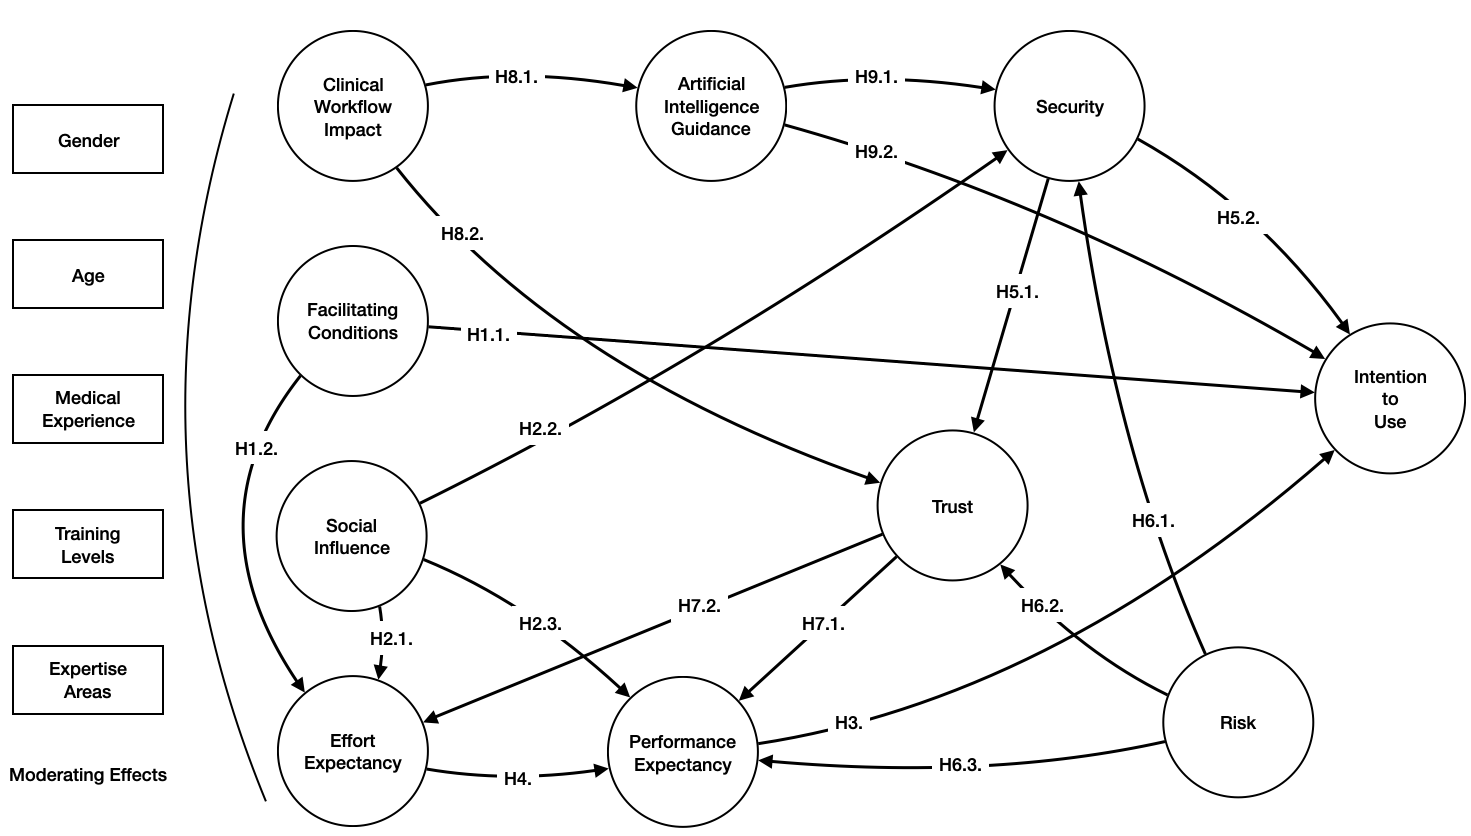
\includegraphics[width=\linewidth]{fig073}
\caption{The proposed research model, comparing the relations between moderating effects, model constructs, and hypotheses. We adapted this proposed research model from the UTAUT theoretical model to explain the actual adoption of AI in the medical imaging workflow. The research model includes 10 factors. We measured each factor with multiple items. Moreover, we adapted all items from extant literature to improve content validity.}
\label{fig:fig073}
\end{figure}
%%%%%%%%%%%%%%%%%%%%%%%%%%%%%%%%%%%%%%%%%%%%%%%%%%%

Content validity is emphasized in the research model through the adaptation of measurement items from existing literature, ensuring that the constructs accurately capture the nuances of \ac{AI} adoption in the medical imaging workflow.
This attention to content validity enhances the reliability and robustness of the research model, enabling a comprehensive evaluation of the factors that influence clinicians' intentions and behaviors regarding the integration of \ac{AI} systems.

In summary, our research model serves as a tailored and comprehensive framework for investigating the adoption of \ac{AI} in the medical imaging workflow.
By integrating core \ac{UTAUT} constructs with domain-specific factors, the model offers a deep understanding of the complex interplay between clinicians, technology, and the healthcare context.
This model is a valuable tool for researchers in the \ac{HCI} and \ac{AI} domains, facilitating a thorough \ac{EFA} driving the successful adoption of \ac{AI} technology in healthcare and supporting the development of effective strategies for its integration.

\section{Demographic Data}
\label{chap:app002003}

In Section~\ref{sec:chap004004002} of Chapter~\ref{chap:chap004}, we provided an overview of the sample demographics (Table~\ref{tab:tab008}) in this study.
This study involved data collected from 322 participants, corresponding to an overall participation rate of 1.9\%.
The distribution of participants varied across different regions, with higher participation observed from individuals in the USA/Canada (25.5\%), Africa (11.2\%), Portugal (10.6\%), and Other-EU Countries (9.9\%).
Conversely, the participation was lower from regions such as the Middle East (8.1\%), Asia (7.5\%), South or Central America (5.9\%), Italy (5.3\%), UK (4.3\%), Non-EU European (3.7\%), New Zealand/Australia (2.8\%), France (1.9\%), Germany (1.9\%), and Spain (1.6\%).
The higher participation from certain regions, such as the USA/Canada and Africa, suggests a potential bias in the sample, as it may not be fully representative of the global population.
The lower participation from regions like Asia and Europe raises the possibility of regional biases, which should be taken into account when generalizing the study findings.
Additionally, the overall participation rate of 1.9\% indicates that the sample size may be relatively small compared to the target population, which could limit the generalizability of the results.
It is important to consider these regional distributions and potential biases when interpreting and applying the findings of the study.

Regarding the demographic characteristics of the participants (N = 322), the sample consisted of slightly more men (59.9\%) than women (38.8\%), with 1.2\% of participants choosing not to disclose their gender (``Prefer not to say'').
In terms of age groups, 12.1\% of participants were between 18 and 29 years old, 29.5\% were between 30 and 39, 22.7\% were between 40 and 49, 23.9\% were between 50 and 59, 10.2\% were older than 59, and 1.6\% preferred not to disclose their age during the questionnaire.
The higher proportion of male participants suggests a potential gender bias in the sample, which should be taken into consideration when generalizing the findings.
Additionally, the distribution across age groups indicates a relatively diverse representation, with participants spanning various age ranges.
However, the lower participation rate in certain age groups, such as those above 59 years old, might introduce a potential age bias.
It is important to be aware of these demographic characteristics and potential biases when interpreting the study results.

In addition to the sample demographics discussed earlier, other demographic data are crucial for this study.
These include the medical experience of participants (Section~\ref{chap:app002003001}), training levels (Section~\ref{chap:app002003002}), and expertise areas (Section~\ref{chap:app002003003}).
The education level of participants is particularly relevant, as it provides insights into the relationships between demographic data and the study variables.
Specifically, among the participants, 34.5\% are specialists in their respective fields, 25.2\% have at least one bachelor's degree, 24.2\% holds a master's degree, and 14\% have a PhD.
The remaining 2.1\% typically consists of students or individuals with academic associate degrees.
These demographic characteristics contribute to a comprehensive understanding of the participant's background and qualifications, shaping their perspectives on \ac{AI} adoption in the medical imaging workflow.

%%%%%%%%%%%%%%%%%%%%%%%%%%%%%%%%%%%%%%%%%%%%%%%%%%%
\begin{table}[htpb]
\resizebox{\columnwidth}{!}{%
\begin{tabular}{cccc}
\hline
\rule{0mm}{4mm}
Demographic                   & Group                    & Frequency & Percentage
\\
\hline
\multirow[t]{3}{*}{Gender}       & Female                    & 125       & 38.8\%     \\
                                 & Male                      & 193       & 59.9       \\
                                 & Other                     & 4         & 1.2        \\
\hline
\multirow[t]{6}{*}{Age}          & 18 - 29                  & 39        & 12.1\%     \\
                                 & 30 - 39                  & 95        & 29.5\%     \\
                                 & 40 - 49                  & 73        & 22.7\%     \\
                                 & 50 - 59                  & 77        & 23.9\%     \\
                                 & > 59                     & 33        & 10.2\%     \\
                                 & N.A.                     & 5         & 1.6\%      \\
\hline
\multirow[t]{7}{*}{Nationality}  & Europe                   & 126       & 39.2\%     \\
                                 & North America            & 82        & 25.5\%     \\
                                 & Africa                   & 36        & 11.2\%     \\
                                 & Middle East              & 26        & 8.1\%      \\
                                 & Asia                     & 24        & 7.5\%      \\
                                 & Central \& South America & 19        & 5.9\%      \\
                                 & Oceania                  & 9         & 2.8\%      \\
\hline
\multirow[t]{5}{*}{Education}    & Specialists              & 111       & 34.5\%     \\
                                 & Bachelor                 & 81        & 25.2\%     \\
                                 & Master                   & 78        & 24.2\%     \\
                                 & PhD                      & 45        & 14\%       \\
                                 & N.A.                     & 7         & 2.1\%      \\
\hline
\multirow[t]{5}{*}{Medical Experience} & Interns            & 24        & 7.5\%      \\
                                       & Juniors            & 26        & 8.1\%      \\
                                       & Middles            & 54        & 16.5\%     \\
                                       & Seniors            & 210       & 65.2\%     \\
                                       & N.A.               & 8         & 2.4\%      \\
\hline
\multirow[t]{3}{*}{Training Levels}    & Doctors            & 132       & 41\%       \\
                                       & Technicians        & 105       & 32.6\%     \\
                                       & Other              & 85        & 26.4\%     \\
\hline
\end{tabular}%
}
\caption{Characteristics of participants for demographic groups with frequency and percentage. The main characteristics are gender, age, nationality, and education.}
\label{tab:tab008}
\end{table}
%%%%%%%%%%%%%%%%%%%%%%%%%%%%%%%%%%%%%%%%%%%%%%%%%%%

The high proportion of specialists suggests that the study sample includes individuals with extensive domain knowledge and expertise, which could positively influence their perceptions and attitudes toward AI systems in the medical imaging workflow.
Furthermore, the diverse educational backgrounds, ranging from bachelor's to doctoral degrees, contribute to a broad representation of perspectives and experiences within the sample.
However, it is essential to acknowledge that the education level distribution within the sample may not fully reflect the broader population.
Potential biases related to educational attainment and expertise areas should be considered when interpreting and generalizing the study findings.
These demographic characteristics play a crucial role in shaping participants' attitudes, perceptions, and potential biases towards \ac{AI} adoption in the medical imaging workflow.

\subsection{Medical Experience}
\label{chap:app002003001}

Regarding medical experience, most participants (65.2\%) in this study are experienced professionals with over 10 years of expertise in their respective fields.
These senior clinicians bring extensive knowledge and practical experience to the study, enriching the discussions and analyses with their wealth of insights and lessons learned from their long-standing careers in healthcare.
An additional 16.5\% of participants fall into the category of middles, representing clinicians with more than 5 years of work experience but less than 10 years.
These individuals have already gained substantial experience in their roles and can offer valuable perspectives based on their mid-level expertise.

On the other hand, 8.1\% of participants are juniors who have recently entered the field and have up to 5 years of experience after completing their medical exams.
As emerging professionals, they provide a fresh perspective and may bring unique insights based on their recent training and exposure to current medical practices.
Additionally, 7.5\% of participants are interns who are actively engaged in their specialty exams.
Their participation offers valuable perspectives on the current state of medical education and training practices, providing a glimpse into the evolving landscape of healthcare.
Combining the junior clinicians and interns, a total of 15.6\% of participants can be categorized as clinical novices.

Lastly, the remaining 2.4\% of participants consist of students and academics who do not fit into the predefined experience groups.
This group brings a unique perspective as they contribute their academic knowledge and potentially offer innovative ideas in the context of \ac{HCI} and \ac{AI} for healthcare.
Their input adds depth to the discussions and enhances the study's ability to explore new avenues and possibilities in the field.
Collectively, the diverse range of participants with varying levels of medical experience enriches the study's findings, providing a comprehensive understanding across the adoption of \ac{AI} in the medical imaging workflow.
By incorporating insights from seasoned experts, mid-level professionals, novices, and academic stakeholders, this research can address the complex dynamics at the intersection of \ac{HCI} and \ac{AI} in healthcare, fostering advancements and improvements in this critical domain.

\subsection{Training Levels}
\label{chap:app002003002}

Regarding participants' training levels, the majority (41\%) are doctors who have completed medical school, obtaining their medical degree.
They have the necessary medical knowledge and expertise to understand the intricacies of the healthcare domain and effectively contribute to the study.
Additionally, 32.6\% of participants are technicians who have received specialized training in medical imaging technology.
Their technical expertise and familiarity with the operational aspects of medical imaging systems provide valuable insights into the practical implementation of \ac{AI} in healthcare settings.
Furthermore, 26.4\% of participants have received training in various disciplines such as nursing, medical physics, or biomedical sciences.

To gain a comprehensive understanding of the clinical workflow, information about the work sector of each participant is also important.
The analysis of the work sectors reveals that 17.39\% of participants work in both the public and private sectors, allowing them to contribute insights from both settings.
Additionally, 39.41\% of participants work exclusively in the public sector, which includes public hospitals or public cancer institutes.
Their experiences in public healthcare institutions provide valuable insights into the challenges and opportunities in the public healthcare landscape.
Another 32.91\% of participants work exclusively in the private sector, such as private clinics or private hospitals, offering unique perspectives from a different organizational context.
The remaining 10.29\% of participants work for companies involved in the healthcare industry, are academics, or have retired from their clinical practice.

Diverse clinician's backgrounds are contributing to a comprehensive understanding of \ac{AI} adoption in healthcare, incorporating insights from various perspectives within the clinical workflow.
By considering the training levels and work sectors of the participants, this study embraces a multidimensional view of \ac{AI} adoption in the medical imaging workflow.
The inclusion of these clinical groups with diverse training backgrounds, combined with insights from both the public and private sectors, ensures a comprehensive exploration of the challenges and opportunities at the intersection of \ac{HCI} and \ac{AI} for healthcare.

\subsection{Expertise Areas}
\label{chap:app002003003}

Regarding expertise areas, the majority of participants (79.2\%) work in the field of radiology.
As experts in medical imaging, their insights are particularly valuable in understanding the integration of \ac{AI} within this domain.
In addition to radiology, it is important to analyze other expertise areas, as they also play a significant role in medical imaging.
For example, 7.1\% of participants specialize in medical intervention, bringing their expertise in interventional procedures to the study.
Similarly, 5.6\% of participants have expertise in oncology, providing valuable insights into the intersection of \ac{AI} and cancer diagnosis or treatment.
Furthermore, 4.3\% of participants specialize in general medicine, offering a broader perspective on \ac{AI} adoption in the context of primary care.

Although with lower participation, it is still important to report the contributions from participants with expertise in other areas.
This includes 2.5\% of participants working in surgery, providing insights into the role of \ac{AI} in surgical procedures.
Additionally, 2.2\% of participants specialize in family medicine, offering insights into the application of AI in a primary care setting. Finally, 1.6\% of participants belong to several other categories, representing a diverse range of specialties that contribute to a comprehensive understanding of AI adoption in the medical imaging workflow.
By considering various expertise areas, this study encompasses a wide range of perspectives from different medical disciplines.
This diverse representation ensures a comprehensive exploration for the design of \ac{AI} systems in healthcare, facilitating the identification of challenges and opportunities in adopting \ac{AI} in medical imaging.

\section{Statistical Analysis}
\label{chap:app002004}

In this section, we delve into the details of the sample characteristics, building upon the information presented in Section~\ref{sec:chap004005} of Chapter~\ref{chap:chap004}.
The analysis of sample characteristics (Table~\ref{tab:tab008}) provides valuable insights into the participant demographics of this study.
The majority of participants were radiology specialists in the age range of 30 to 39 years, indicating a specific professional profile.
These participants exhibited early experience in their field, with an average of over ten years of expertise.
Their primary employment was within the public sector, highlighting their involvement in healthcare services in government-funded institutions.
Most respondents (66.1\%) reported analyzing medical imaging exams daily, indicating a regular and ongoing involvement in this practice.
The majority reported a daily involvement in this practice, while a smaller percentage indicated varying frequencies, such as 3--4 days a week (7.8\%), 2--3 days a week (3.7\%), or once a week (3.7\%).
Additionally, a notable portion (18.7\%) reported conducting such analysis monthly or as needed, reflecting a less frequent engagement.

The findings indicate a diverse range among the participants in terms of the duration of their experience in analyzing patients with medical imaging exams.
Approximately 28\% reported having more than 20 years of experience, while 27\% had less than five years.
The remaining participants fell into the categories of 6--10 years (17.1\%), 11--15 years (15.5\%), and 16--20 years (12.4\%).
These varied experience levels contribute to the study cohort's richness and diversity of perspectives.

Participants were probed about their familiarity with \ac{AI} systems and patterns of utilization, yielding insightful findings.
While a significant portion (42.5\%) displayed knowledge about \ac{AI}, they had not yet engaged with the technology themselves.
Approximately 27\% had attempted to use \ac{AI} systems sporadically, and 19.3\% reported regular utilization.
Surprisingly, 11.2\% of participants indicated a complete lack of awareness regarding \ac{AI}, highlighting the need for enhanced education and awareness initiatives in this domain.
These findings emphasize the importance of promoting knowledge and providing comprehensive guidance to ensure the seamless integration of \ac{AI} systems in the healthcare domain.

\subsection{Model Assumptions and Fit Analysis}
\label{chap:app002004001}

We checked the \ac{SEM} assumptions, where all variables showed a normal distribution, based on a visual inspection of box plots and histograms.
Residuals showed a normal distribution with no relation between residuals and predictors~\cite{CALISTO2022102922}.
The model's overall fit was good, with all the relevant \acp{GFI} higher than the recommended threshold of 0.90 for \acp{AGFI} and 0.95 for other indices~\cite{doi:10.1504/IJMDA.2017.087624, SUMAK2016602}.

Under this study, the \ac{GFI} = 0.824, the \ac{AGFI} was 0.784, the \ac{CFI} = 0.909, the \ac{NFI} was 0.861, and the \ac{TLI} = 0.896 reported from our analysis.
Although \ac{GFI} ($GFI = 0.824 < 0.90$), \ac{AGFI} ($AGFI = 0.784 < 0.80$), and \ac{TLI} test ($TLI = 0.896 < 0.90$) are slightly lower than the recommended levels, studies have shown that sample size impacts these fit indices~\cite{KHALILZADEH2017460, doi:10.1080/00273171.2019.1602503, ZHOU2010760}.
Some of these studies show the downward bias of the previously mentioned indices when the degree of freedom values increase in comparison to the sample size of the model~\cite{doi:10.1080/00273171.2019.1602503}.
Indeed, the ratio of the test statistic ($\chi^2$) to the degree of freedom ($df$) was lower than 3.0 as recommended ($\chi^2$ / $df$ $= 2.587 < 3.0$) in the literature.
Pairwise with the \ac{RMSEA} ($RMSEA = 0.073 < 0.08$), both indicated an acceptable model fit~\cite{ZHOU2010760}.

The model's test statistic ($\chi^2$) was significant due to the sample size.
Based on Hoelter index~\cite{CALISTO2022102922}, the sample size of 138 is sufficient, and the sample of 322 seems adequate for the sophisticated study model.
Additionally, the \ac{SRMR} was also good, at 0.083, above the threshold ($SRMR = 0.083 > 0.06$) for a good overall fit.

\subsection{Model Validation and Assessment}
\label{chap:app002004002}

In this section, we delve into the measurement model to assess the quality and reliability of the measured constructs (Section~\ref{sec:chap004005002}), following the satisfactory model fit observed in the previous analysis.
The focus now shifts towards refining the measurement items and evaluating the model fit, validity, and reliability of the measurement scales employed.
To this end, we present the results of the \ac{CFA}, providing insights into the measurement properties of the constructs.
The comprehensive findings are summarized in Table~\ref{tab:tab009}, which serves as a reference for the subsequent analyses and discussions.

%%%%%%%%%%%%%%%%%%%%%%%%%%%%%%%%%%%%%%%%%%%%%%%%%%%
\begin{table*}
\resizebox{\textwidth}{!}{%
\begin{tabular}{ccccccccccc}
\hline
Measure & Impact & Guidance & PerfExp & EffExp & SocInf & FacCond & IntUse & Security & Risk & Trust \\ \hline
alpha   & 0.57   & 0.88     & 0.87    & 0.89   & 0.73   & 0.80    & 0.94   & 0.83     & 0.84    & 0.88  \\
CR      & 0.57   & 0.88     & 0.89    & 0.89   & 0.74   & 0.79    & 0.93   & 0.82     & 0.84    & 0.88  \\
AVE     & 0.40   & 0.65     & 0.72    & 0.73   & 0.49   & 0.55    & 0.78   & 0.60     & 0.64    & 0.70  \\ \hline
\end{tabular}%
}
\caption{The abbreviated constructs are as follows: Clinical Workflow Impact (Impact); AI Guidance (Guidance); Performance Expectancy (PerfExp); Effort Expectancy (EffExp); Social Influence (SocInf); Facilitating Conditions (FacCond); Behavior Intention to Use (IntUse); Perceived Security (Security); Perceived Risk (Risk); Perceived Trust (Trust). Moreover, the measure abbreviations are: Cronbach alpha (alpha); Composite Reliability (CR); Average Variance Extracted (AVE).}
\label{tab:tab009}
\end{table*}
%%%%%%%%%%%%%%%%%%%%%%%%%%%%%%%%%%%%%%%%%%%%%%%%%%%

Convergent validity shows whether each factor can be reflected by its items~\cite{CALISTO2022102922}.
To this end, all loadings were significant at alpha level ({\it p-value} = 0.000), and the minimum loading was 0.57, with most loadings higher than 0.8, which indicates good convergent validity~\cite{CALISTO2022102922}.
Each item loaded significantly ({\it p-value} $<$ 0.001) on its underlying construct in all cases.
On the other hand, discriminant validity reflects whether two factors are statistically different~\cite{CALISTO2022102922}.
For that, we examined both the convergence and discriminant validity of the model, measuring the reliability of each measure and each construct and the \ac{AVE} for each construct.

We compared the shared variance across constructs with the \ac{AVE} from the individual construct to examine discriminant validity.
The shared variety between constructs was lower than the \ac{AVE} from the individual constructs (Table~\ref{tab:tab009}), confirming discriminant validity.
In the end, we checked the measurement model for the \acl{CR} ($CR = 0.95$), which indicated good measurement reliability of our measurement model~\cite{doi:10.1504/IJMDA.2017.087624, SUMAK2016602}.

To conclude, the measurement model demonstrated adequate reliability, convergent validity, and discriminant validity.
However, given the complex relationships across the model's factors, we should consider the moderating effects on other variables.
Expressly, we can reasonably assume that the model has unexpected moderating relationships.
Hence, recognizing moderating effects for demographics (Section~\ref{sec:chap004005005}) across the factors is particularly important in this study and must be further reported.

\subsection{Parallel Analysis for Determining Factor Retention}
\label{chap:app002004003}

In this section, we present a comprehensive analysis of the parallel analysis results, which aim to determine the optimal number of factors to retain in the measurement model.
These results further build upon the findings discussed in Section~\ref{sec:chap004005003}, providing a detailed understanding of the factor retention process.
Parallel analysis, as described by Luo et al.~\cite{doi:10.1080/10705511.2019.1615835}, is a valuable technique that compares the eigenvalues obtained from the analysis with simulated eigenvalues derived from the number of items and sample size.
The insights contribute to a more refined and accurate measurement model, ensuring that the retained factors capture the underlying dimensions of the construct in a meaningful and comprehensive way.
In turn, this analysis strengthens the validity and reliability of the research findings in the context of \ac{HCI} and \ac{AI} for healthcare.

The scree plot in Figure~\ref{fig:fig093} offers valuable guidance in determining the number of factors to retain.
We observe significant changes in effect size, suggesting potential breakpoints for a number of factors.
However, it is crucial to consider the line limits of the parallel analysis to make informed decisions.
For example, the difference between the first components supports an optimal eigenvalue size of four.
Furthermore, a more conclusive difference is observed when comparing components five and six, as well as six and seven.
Conversely, components eight and nine fall below the retention line, indicating that the decision to retain an item for a factor or overall model is generally arbitrary~\cite{CALISTO2022102922}.

%%%%%%%%%%%%%%%%%%%%%%%%%%%%%%%%%%%%%%%%%%%%%%%%%%%
\begin{figure}[htpb]
\centering
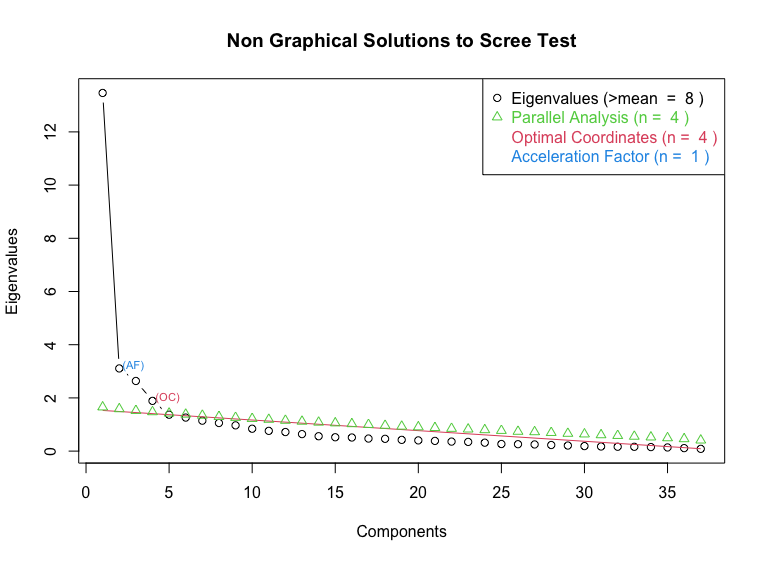
\includegraphics[width=0.855\linewidth]{fig093}
\caption{Scree plot of eigenvalues with the eigenvalues greater than one rule, elbow bend, and intersecting lines.}
\label{fig:fig093}
\end{figure}
%%%%%%%%%%%%%%%%%%%%%%%%%%%%%%%%%%%%%%%%%%%%%%%%%%%

Overall, the parallel analysis results provide valuable insights into determining the appropriate number of factors to retain in the measurement model.
This analysis contributes to the robustness and validity of our research in the intersection of \ac{HCI} and \ac{AI} for healthcare.
Therefore, further enhancing our understanding of the underlying factors in the model.

\subsection{Evaluation of the Structural Model and Findings}
\label{chap:app002004004}

In this study, we employed \ac{SEM} to analyze our data (Section~\ref{sec:chap004005004} of Chapter~\ref{chap:chap004}), as the measurement model achieved an overall fit.
\ac{SEM} allows for evaluating how well the data align with the theoretical measurement of the model~\cite{doi:10.1080/10705511.2017.1401932}.
Building upon the proposed research model, we introduced two new constructs:
(1) Clinical Workflow Impact; and
(2) \ac{AI} Guidance.
Furthermore, we extended the model by examining the interactions between these constructs and variables such as security, trust, and behavioral intention to use.
We estimated the hypothesized causal paths depicted in Figure~\ref{fig:fig073} to assess the structural relationships.
The results presented in Table~\ref{tab:tab011} demonstrate that the majority of hypotheses are supported ({\it p-value} $<$ 0.10).
However, we observed that hypotheses {\bf H6.1}, {\bf H6.3}, and {\bf H7.1} did not meet this criterion.
By examining these structural relationships, we gain insights into the impact of \ac{AI} technologies on the adoption and usage in healthcare settings.

%%%%%%%%%%%%%%%%%%%%%%%%%%%%%%%%%%%%%%%%%%%%%%%%%%%
\begin{table}[htpb]
\resizebox{\columnwidth}{!}{%
\begin{tabular}{lrrrrrl}
\hline
Hypotheses & \multicolumn{1}{l}{b} & \multicolumn{1}{l}{StdError} & \multicolumn{1}{l}{z-value} & \multicolumn{1}{l}{p-value} & \multicolumn{1}{l}{beta} & Supported \\
\hline
\textbf{H1.1.} & 0.313  & 0.053 & 5.912  & 0.000 & 0.349  & Yes ***                  \\
\textbf{H1.2.} & 0.432  & 0.08  & 5.393  & 0.000 & 0.375  & Yes ***                  \\
\textbf{H2.1.} & 0.268  & 0.133 & 2.015  & 0.044 & 0.211  & Yes **                   \\
\textbf{H2.2.} & 0.432  & 0.08  & 5.393  & 0.000 & 0.375  & Yes ***                  \\
\textbf{H2.3}  & 0.239  & 0.067 & 3.554  & 0.000 & 0.243  & Yes ***                  \\
\textbf{H3.}   & 0.327  & 0.068 & 4.81   & 0.000 & 0.264  & Yes ***                  \\
\textbf{H4.}   & 0.466  & 0.061 & 7.653  & 0.000 & 0.603  & Yes ***                  \\
\textbf{H5.1.} & 0.701  & 0.078 & 9.012  & 0.000 & 0.715  & Yes ***                  \\
\textbf{H5.2.} & 0.239  & 0.06  & 4.005  & 0.000 & 0.226  & Yes ***                  \\
\textbf{H6.1.} & -0.016 & 0.049 & -0.326 & 0.744 & -0.02  & \textcolor{red}{No}      \\
\textbf{H6.2.} & -0.098 & 0.059 & -1.672 & 0.095 & -0.124 & Yes *                    \\
\textbf{H6.3.} & -0.031 & 0.033 & -0.962 & 0.336 & -0.046 & \textcolor{red}{No}      \\
\textbf{H7.1.} & 0.009  & 0.045 & 0.197  & 0.844 & 0.01   & \textcolor{red}{No}      \\
\textbf{H7.2.} & 0.375  & 0.062 & 6.014  & 0.000 & 0.333  & Yes ***                  \\
\textbf{H8.1.} & -0.494 & 0.09  & -5.512 & 0.000 & -0.487 & Yes ***                  \\
\textbf{H8.2.} & 0.176  & 0.092 & 1.92   & 0.055 & 0.179  & Yes *                    \\
\textbf{H9.1.} & 0.459  & 0.067 & 6.861  & 0.000 & 0.464  & Yes ***                  \\
\textbf{H9.2.} & 0.336  & 0.055 & 6.151  & 0.000 & 0.322  & Yes ***                  \\
\hline
\end{tabular}%
}
\caption{Summary of hypothesis tests. The variables assigned to the significance values are as follows: *** significant at level $\alpha = 0.01$; ** significant at level $\alpha = 0.05$; and * significant fixed at level $\alpha = 0.10$.}
\label{tab:tab011}
\end{table}
%%%%%%%%%%%%%%%%%%%%%%%%%%%%%%%%%%%%%%%%%%%%%%%%%%%

The coefficient of determination ($R^2$), also referred to as \ac{SMC}, was employed to assess the explanatory power and predictive accuracy of the measurement model (Table~\ref{tab:tab010}).
This analysis builds upon the findings discussed in Section~\ref{sec:chap004005004}, where we presented an overview of the model's fit.
The $R^2$ coefficient, ranging from 0 to 1, provides insights into the proportion of variance in the dependent variable that can be accounted for by the independent variables~\cite{doi:10.1080/10705511.2017.1401932}.
In our study, we observed varying explanatory power levels across the measurement model constructs.

A higher $R^2$ value indicates a greater extent to which the model accounts for the variability in the dependent variable.
In our study, the behavioral intention construct exhibited the highest $R^2$ value of 0.681 (Table~\ref{tab:tab010}), indicating that a substantial amount of variance in the dependent variable can be attributed to the proposed model.
Conversely, the \ac{AI} Guidance construct had the lowest $R^2$ value of 0.238, followed by security with an $R^2$ value of 0.397. These relatively lower values can be attributed to their close association with independent variables and the inherent nature of these constructs, grounded in a clinician's belief in \ac{AI} systems.
Furthermore, the performance expectancy construct yielded a coefficient of determination ($R^2$) value of 0.595, denoting a substantial amount of variance explained.
Similarly, the effort expectancy and trust constructs exhibited acceptable $R^2$ values of 0.496 and 0.465, respectively (Table~\ref{tab:tab010}).
These findings are consistent with prior research results~\cite{KHALILZADEH2017460}, supporting the validity and reliability of our measurement model.

%%%%%%%%%%%%%%%%%%%%%%%%%%%%%%%%%%%%%%%%%%%%%%%%%%%
\begin{table}[htpb]
\resizebox{\columnwidth}{!}{%
\begin{tabular}{llrrrl}
\hline
Construct                   & Item        & \multicolumn{1}{l}{Alpha} & \multicolumn{1}{l}{StdError} & \multicolumn{1}{l}{z-value} & p-value \\ \hline
Clinical Workflow Impact & Impact\_1   & 0.53 & 0.080 & 6.615  & 0.000 \\
Alpha = 0.57                & Impact\_2   & 0.75  & 0.079    & 9.499   & 0.000   \\ \hline
AI Guidance              & Guidance\_1 & 0.36 & 0.035 & 10.209 & 0.000 \\
Alpha = 0.88             & Guidance\_2 & 0.29 & 0.028 & 10.102 & 0.000 \\
R2 = 0.238                  & Guidance\_3 & 0.19  & 0.026    & 7.262   & 0.000   \\
                            & Guidance\_4 & 0.32  & 0.033    & 9.683   & 0.000   \\ \hline
Performance Expectancy      & PerfExp\_1  & 0.45                      & 0.039                        & 11.606                      & 0.000   \\
Alpha = 0.87                & PerfExp\_2  & 0.14                      & 0.019                        & 7.186                       & 0.000   \\
R2 = 0.595                  & PerfExp\_3  & 0.08                      & 0.018                        & 4.382                       & 0.000   \\ \hline
Effort Expectancy           & EffExp\_1   & 0.16                      & 0.022                        & 7.335                       & 0.000   \\
Alpha = 0.89                & EffExp\_2   & 0.19                      & 0.021                        & 8.615                       & 0.000   \\
R2 = 0.496                  & EffExp\_3   & 0.25                      & 0.025                        & 9.821                       & 0.000   \\ \hline
Social Influence            & SocInf\_1   & 0.57                      & 0.054                        & 10.464                      & 0.000   \\
Alpha = 0.73                & SocInf\_2   & 0.68                      & 0.066                        & 10.24                       & 0.000   \\
                            & SocInf\_3   & 0.35                      & 0.047                        & 7.356                       & 0.000   \\ \hline
Facilitating Conditions     & FacCond\_1  & 0.56                      & 0.06                         & 9.284                       & 0.000   \\
Alpha = 0.80                & FacCond\_2  & 0.57                      & 0.061                        & 9.45                        & 0.000   \\
                            & FacCond\_3  & 0.41                      & 0.046                        & 8.932                       & 0.000   \\ \hline
Behavioral Intention to Use & IntUse\_1   & 0.16                      & 0.017                        & 9.576                       & 0.000   \\
Alpha = 0.94                & IntUse\_2   & 0.13                      & 0.015                        & 8.496                       & 0.000   \\
R2 = 0.681                  & IntUse\_3   & 0.15                      & 0.016                        & 9.761                       & 0.000   \\
                            & IntUse\_4   & 0.19                      & 0.019                        & 9.856                       & 0.000   \\ \hline
Security                    & Security\_1 & 0.41                      & 0.041                        & 10.055                      & 0.000   \\
Alpha = 0.83                & Security\_2 & 0.14                      & 0.025                        & 5.621                       & 0.000   \\
R2 = 0.397                  & Security\_3 & 0.39                      & 0.037                        & 10.537                      & 0.000   \\ \hline
Risk                        & Risk\_1  & 0.36                         & 0.049                        & 7.342                       & 0.000   \\
Alpha = 0.84                & Risk\_2  & 0.57                         & 0.06                         & 9.48                        & 0.000   \\
                            & Risk\_3  & 0.34                         & 0.047                        & 7.114                       & 0.000   \\ \hline
Trust                       & Trust\_1    & 0.30                      & 0.031                        & 9.762                       & 0.000   \\
Alpha = 0.88                & Trust\_2    & 0.19                      & 0.025                        & 7.606                       & 0.000   \\
R2 = 0.465                  & Trust\_3    & 0.21                      & 0.029                        & 7.385                       & 0.000  \\ \hline
\end{tabular}%
}
\caption{The measuring model with: Clinical Workflow Impact ({\bf Impact}); AI Guidance ({\bf Guidance}); Performance Expectancy ({\bf PerfExp}); Effort Expectancy ({\bf EffExp}); Social Influence ({\bf SocInf}); Facilitating Conditions ({\bf FacCond}); Behavioral Intention to Use ({\bf IntUse}); {\bf Security}; {\bf Risk}; and {\bf Trust}. The computed measurements are {\bf Alpha}, Standard Error ({\bf StdError}), {\bf z-value}, and {\bf p-value}.}
\label{tab:tab010}
\end{table}
%%%%%%%%%%%%%%%%%%%%%%%%%%%%%%%%%%%%%%%%%%%%%%%%%%%

\subsection{Moderating Effects and Measurement Invariance Analysis}
\label{chap:app002004005}

To investigate demographic moderator effects, we conducted a moderating analysis using the split sample approach \cite{LI2021106581, LI2021106929}.
This approach uses a pre-established moderator level, which emerges naturally from data and cannot be modified by the study.
For instance, the nationality of a clinician, gender, or age variables is a form of different moderator levels.
We tested the moderator effects of gender (F/M), age (divided into two groups $<$ 30 and $\geq$ 30), nationality (grouped into developed and developing countries), education (higher and advanced education), and a proxy of clinical knowledge (expert {\it vs.} novice) for working with medical imaging technologies, which was calculated from a combination of medical experience (Section~\ref{chap:app002003001}), training levels (Section~\ref{chap:app002003002}), and expertise areas (Section~\ref{chap:app002003003}).

We classified senior and middle radiology doctors as experts working with medical imaging technologies.
Similarly, we also consider senior and middle radiology technicians as experts with knowledge of working with these technologies.
On the contrary, we consider novice knowledge of all juniors and interns independent of being doctors, technicians, or another different training level.
We also considered all clinicians not working directly in radiology expertise as having novice knowledge of medical imaging technologies.

We tested the moderating effects (Table~\ref{tab:tab012} of Section~\ref{sec:chap004005005}) of the above variables by comparing, between the different groups, the path coefficients produced for each moderator after testing for measurement invariance using $X^2$ difference tests, and the fit indices.
Furthermore, we tested invariance for factor structure, loading, residuals, and means.
The model supported enough evidence of measurement invariance at {\it p-value} $<$ 0.001 significance.
These findings contribute to a deeper understanding of various factors impact on the research model.

\subsection{Summary}
\label{chap:app002004006}

Overall, the results from this study demonstrate that our research model explains 68.1\% (Table~\ref{tab:tab010}) of the intention to use \ac{AI}.
Compared to other empirical results~\cite{LIU2022107026, CALISTO2022102922} of \ac{UTAUT} models, which are explaining a variance between 51.5\%~\cite{LIU2022107026} and 66.4\%~\cite{CALISTO2022102922}.
Notice that studies related to the use of \ac{AI} are still scarce, exhibiting a low variance below 70\%.
However, the extended model in this study has demonstrated a similar achievement in terms of good explanatory and predictive power ({\it i.e.}, 70\% approx.) of the model.
Our model has enough explanatory and predictive power, including new constructs regarding the willingness to follow the {\it AI guidance} ({\it i.e.}, recommendations) and the extent to which \ac{AI} positively {\it impacts the clinical workflow}.
Hence, shaping a more complex network of interrelated causal relationships is not present in the original \ac{UTAUT} models.
This idea borrowed from the literature~\cite{KHALILZADEH2017460, SIGERSON201887} in which it extends both \ac{UTAUT} and \ac{UTAUT}2 models with the inclusion of other influential constructs, increasing the explanatory power of the model while keeping parsimony.

In line with other authors~\cite{CALISTO2022102922}, we reduced the number of items in some constructs while preserving reliability.
Thus, condensing  the scale even further than the above research~\cite{KHALILZADEH2017460}.
According to the literature recommendations \cite{SIGERSON201887}, we were able to retain the factors with only several items retaining validity, reliability, and correlation.

\section{Synthesis and Reflection}
\label{chap:app002005}

In this section, we provide a detailed analysis of the obtained results, discussing their significance and implications for the research.
For a more concise overview of our findings, please refer to Section~\ref{sec:chap004006} of Chapter~\ref{chap:chap004}.
The study introduced a theoretical research model that examined the influence of security, risk, and trust on the acceptance of \ac{AI} recommendations, building upon the \ac{UTAUT} model.
The results (Section~\ref{sec:chap004005}) strongly support the validity and reliability of the proposed acceptance model (Figure~\ref{fig:fig074}), which accounted for 68.1\% of the variance in the behavioral intention to use an AI system.
These findings hold essential theoretical and practical implications, as discussed in the subsequent sections.

\subsection{Main Findings and Implications}
\label{chap:app002005001}

The findings of this study show that facilitating conditions are positively predicting the intention to use \ac{AI} ({\bf H1.1.}) in the clinical workflow.
However, facilitating conditions not only affect usage behavior in the original UTAUT model, but also supports the positive effect of facilitating conditions on behavioral intention.
On the other hand, the study results show a significant relationship between facilitating conditions and effort expectancy ({\bf H1.2.}).
Additionally, the role of facilitating conditions increased significantly (Table~\ref{tab:tab012}) with the specific moderating effect of {\it males} for both intention to use and effort expectancy.
Overall, the results of the study demonstrate that facilitating conditions in the clinical workflow would impact attitude and intention to use \ac{AI} systems (Section~\ref{sec:chap004006001} of Chapter~\ref{chap:chap004}), as well as a positive impact on belief and usage of these systems.

The direct impact of social influence on effort expectancy ({\bf H2.1.}), perceived security ({\bf H2.2.}), and performance expectancy ({\bf H2.3.}) of using \ac{AI} systems on the clinical workflow is significant.
Our results suggest that social influence positively impacts the adoption of \ac{AI} systems.
These findings indicate that the more \ac{AI} systems decrease the effort to diagnose a patient while increasing clinicians' performance in the clinical workflow, the more it influences the medical community.
At the same time, perceived security is also influencing the medical community.
Meaning that the more the medical community reports \ac{AI} algorithms as secure, the more clinicians are willing to adopt \ac{AI} systems in their clinical workflow.
However, concerning the moderating effects (Table~\ref{tab:tab012}), our results are indicating that the groups of {\it younger clinicians} with {\it novice knowledge} are not significantly related to their social influence in the technology when considering the factors of perceived security and performance expectancy.

The results show that the clinicians' intention to use an \ac{AI} system is positively affected by performance expectancy ({\bf H3.}), which supports the existing research on the behavioral intention to adopt novel health technologies~\cite{WU2021106840}.
In addition, for the groups of male expert clinicians ({\it e.g.}, typically {\it older males clinicians} and clinicians with {\it expert knowledge}), the impact of \ac{AI} on the clinical workflow is significantly affected by performance expectancy.
Performance expectancy indicates that this behavioral intention is a key determinant for adoption, as long as the final decision-making performs better with \ac{AI} than with traditional diagnosis~\cite{LIN2021e486}.
Another essential requirement is the ability of \ac{AI} to mimic human rationale with interactive assistance.
By providing direct, interactive assistance adapted to each reported group of clinicians and simple operations for supporting the final decision-making, intelligent agents are enabling clinicians to use it more easily~\cite{CALISTO2021102607}.
Thus, our findings highlight the potential of \ac{AI} to optimize the clinical workflow and empower clinicians to provide enhanced patient care.

Effort expectancy positively affects the performance expectancy construct ({\bf H4.}).
If clinicians think that \ac{AI} assistance can provide an easy, precise, and understandable recommendation, they are more likely to expect higher performance from the system.
Theoretically, this adds a new view to \ac{UTAUT} research.
As the ease of use for intelligent agents increases, performance expectancy for \ac{AI} systems will become more positive.
Besides, there is a significant decrease in terms of mediating effects for groups of {\it female}, {\it young clinicians}, as well as clinicians with {\it advanced education} and {\it novice knowledge} on the medical imaging practice (Table~\ref{tab:tab012}).
Hence, the research community should ensure these intelligent agents cover the above group characteristics.
Our results highlight the requirements to consider clinicians' diversity and unique needs when integrating \ac{AI} into the clinical workflow.
Intelligent agents must go beyond being user-friendly for most clinicians and also address {\it variations in expertise}, {\it educational background}, and {\it familiarity} with \ac{AI} systems for medical imaging diagnosing.
By recognizing these group differences and mediating effects, \ac{HCI} and \ac{AI} communities can develop tailored approaches for successfully integrating \ac{AI} systems in healthcare.
These findings emphasize the importance of design interventions and usability studies to effectively integrate \ac{AI} into the clinical workflow.

Our findings highlight the strong influence of security on clinicians' trust in \ac{AI} systems ({\bf H5.1.}).
Moreover, we observed significant effects on specific groups, such as a decrease in trust among {\it females}, {\it young clinicians} with {\it advanced education} but {\it novice knowledge} in medical imaging.
Notably, the role of attitude becomes increasingly crucial for {\it males}, {\it older clinicians}, and {\it developed countries} with {\it higher education} and {\it expert knowledge}, as they exhibit higher levels of trust and positive behavioral intention ({\bf H5.2.}).
These results emphasize the need for the research community to focus on adopting \ac{AI} in the medical imaging domain.
Specifically, it is crucial to address security concerns and gain a deeper understanding of the factors influencing attitudes and intentions among different groups of clinicians.
By doing so, researchers can ensure the successful integration of \ac{AI} systems and promote their widespread acceptance and utilization in healthcare settings.

Although some of our hypotheses ({\it e.g.}, {\bf H6.1.} and {\bf H6.3.}) are not supported for perceived risk, our empirical findings demonstrate that it is an essential construct for some groups of the moderating effects.
Perceived risk is related to the level of \ac{AI} performance ({\bf H6.3.}) concerning clinician's expectations, where the groups of {\it females}, and clinicians working in {\it developed countries} (Table~\ref{tab:tab012}) are showing small, yet, significant values.
It is related to the degree to which clinicians believe using the technology will improve their diagnostic performance and final patient care.
Specifically, it is related to the possibility of \ac{AI} misdiagnosing a patient and not performing as expected.
Therefore, failing to deliver more accurate decision-making in the clinical workflow.
Addressing these concerns is crucial for successfully integrating \ac{AI} in the clinical workflow and improving decision-making accuracy.

Perceived trust in patient's privacy ({\bf H6.2.}) is also related to perceived risk, but this time only significant for the groups of {\it female clinicians}.
Here, perceived trust pertains to clinicians' concern over the misuse or unwanted disclosure of their patients' information.
Another critical empirical finding of this study is that perceived risk negatively impacts perceived security ({\bf H6.1.}).
Depending on the group of the moderating effects, clinicians would feel insecure using \ac{AI} if they perceive a low performance of the model and risk their trust in patients' privacy.
From another perspective, the perceived trust of clinicians within this new \ac{AI} paradigm would increase by improving the algorithm performance and successful implementation of the diagnostic tasks.
These results provide valuable insights for both \ac{AI} and \ac{HCI} communities, guiding efforts to address privacy concerns and improve user trust in \ac{AI} systems.

Including the construct for the clinical workflow, impact enabled us to understand if there was a significant but weak impact on trust ({\bf H8.2.}).
Specially, when considering the moderating effects (Table~\ref{tab:tab012}).
Our results show that for some groups ({\it e.g.}, {\it young clinicians} and clinicians with {\it novice knowledge} in the medical imaging field), the clinical workflow impact is not significantly related to their trust in the technology.
According to our results, the same weak link between the influence of trust on performance expectancy ({\bf H7.1.}) and effort expectancy ({\bf H7.2.}), is clear on groups of {\it young} and {\it novice clinicians}.
On the contrary, for the groups of expert clinicians ({\it e.g.}, typically {\it older clinicians} and clinicians with {\it expert knowledge}), the impact of \ac{AI} on the clinical workflow is significantly related to the trust on the system.
Consequently, our findings accentuate the nuanced nature of trust in different clinician groups and emphasize the importance of tailoring approaches to build trust among diverse users.

Comprehensively, the role of \ac{AI} guidance on security ({\bf H9.1.}) and behavioral intention ({\bf H9.2.}) retained significant regardless of moderator variables.
However, the new \ac{AI} guidance construct ({\it i.e.}, the aim of clinicians to follow an \ac{AI} recommendation) on security ({\bf H9.1.}), decreases with all moderating effects except for {\it males} and {\it older clinicians}.
Similarly, the role of \ac{AI} guidance on intention to use ({\bf H9.2.}), decreases with all moderating effects.
Still, this time except {\it males}, {\it older clinicians}, and clinicians with {\it expert knowledge}.
Therefore, these findings underscore the importance of customizing \ac{AI} guidance to align with the needs and preferences of diverse user groups in healthcare settings.

\subsection{Design Considerations}
\label{chap:app002005002}

Given the increasing demand for intelligent agents in the clinical workflow of medical imaging, our findings offer valuable guidelines and implications for design considerations.
They shed light on key aspects to ensure the successful implementation of \ac{AI} technology for patient diagnosis.
Trust emerges as a critical factor in accepting intelligent agents, aligning with the insights of other researchers~\cite{LIU2022107026}.
To facilitate user engagement and acceptance, building and maintaining clinicians' trust should be a top priority.

In this section, we present design considerations that guide the development of intelligent agents in medical imaging.
These recommendations, summarized in Section~\ref{sec:chap004006002}, emphasize informative \ac{AI} guidance and personalized communication to empower clinicians.
Considering case variability and enhancing \ac{AI} system usability and functionality foster trust and acceptance among clinicians.

\vspace{1.50mm}

\noindent
To that end, we propose the following design considerations based on our study:

\vspace{0.05mm}

\begin{enumerate}
\item {\bf Informative \ac{AI} Guidance}: Intelligent agents should provide clinicians with clear information about the consequences of following \ac{AI} guidance and its impact on the clinical workflow. Clinicians should have control over their choices, empowering their decision-making process.
\item {\bf Personalized Communication}: \ac{AI} systems should consider demographic data and adapt the communication style of the intelligent agent based on factors, {\it e.g.}, gender, age, and country development categories of clinicians. Customizing the communication approach can enhance user engagement and address specific user characteristics and preferences.
\item {\bf Case Variability Consideration}: \ac{AI} systems should consider the variability of different medical cases, individual conditions, and specific needs using diverse AI techniques. The ability to adapt to individual cases and tailor the \ac{AI} results to specific contexts can increase the relevance and usefulness of \ac{AI} guidance.
\item {\bf Usability and Functionality Enhancement}: Designers and developers should focus on improving the ease of use and usefulness of \ac{AI} systems to enhance clinicians' perceived security, perceived risk, and trust. User satisfaction and behavioral intention are outcomes of trust, and ease of use and usefulness are key antecedents of user confidence. By prioritizing these aspects, \ac{AI} systems can foster greater trust and acceptance among clinicians.
\end{enumerate}

Similar to the work of Liu et al.~\cite{LIU2022107026}, our results show how intelligent agents may optimize their control over a decision while informing the consequences of it.
As a (1) first recommendation to introduce an \ac{AI} algorithm successfully in these clinical workflows, intelligent agents must derive efficient representations ({\it e.g.}, explanations), and use them to specify each patient case.
By providing efficient representations and control, clinicians will trust more \ac{AI} guidance, with a higher feeling of security and less risk in their decision.

For the (2) second recommendation, our results show how clinicians behave and perceive differently regarding several demographic groups.
We found differences in behavior between gender, age, and country development categories.
Hence, it is essential to adapt intelligent agents' communication depending on each situation's specific characteristics.
For example, clinicians from developed countries usually have access to cutting-edge technology and, thus, are more aware of \ac{AI} technology. However, clinicians from underdeveloped countries are typically less familiar with it.
This is an important finding and recommendation in our study, as the level of \ac{AI}-based communication must be adapted to groups of clinicians.
Considering these variations when designing intelligent agents can enhance their effectiveness and acceptance among diverse clinician populations.

As a (3) third recommendation identical to the last one, we found personalizing how intelligent agents report \ac{AI} results attractive.
\ac{AI} system designers and developers should consider the variability of different medical cases and embrace the individual needs of clinicians with varied \ac{AI} techniques.
We must pay attention to individual conditions, such as medical experience ({\it e.g.}, expert {\it vs.} novice knowledge), training levels, and expertise areas.
For instance, expert clinicians may be more susceptible than novice clinicians (and vice versa) to an \ac{AI} technique trained on a dataset of images or trained with patients' medical histories.
By tailoring the reporting of \ac{AI} results to align with individual clinician characteristics, we can enhance their understanding and acceptance of the technology.

Finally, our (4) fourth recommendation denotes how \ac{AI} designers and developers should enhance new intelligent agents' usability and functionality.
Although we already reported other salient design recommendations, increasing the ease of use and usefulness of an intelligent agent is of chief importance for \ac{AI} adoption.
Whereas user satisfaction and behavioral intention are consequences of trust~\cite{LIU2022107026, LV2022106993}, ease of use and usefulness are significant antecedents of user confidence.
Therefore, prioritizing usability and functionality improvements can significantly enhance clinicians' perceived security, risk, and trust in \ac{AI}, fostering greater acceptance and adoption.

\section{Final Remarks}
\label{chap:app002006}

In this appendix, we thoroughly analyzed our research findings, focusing on the acceptance and adoption of \ac{AI} systems within the clinical workflow of medical imaging.
This appendix builds upon the summarized conclusions (Section~\ref{sec:chap004008}) presented in Chapter~\ref{chap:chap004}.
It delves deeper into investigating trust, security, and risk, among other factors.
The primary focus is understanding their impact on clinicians' intention to use \ac{AI} and the resulting implications for the clinical workflow.
The comprehensive nature of our results offers valuable insights and practical implications for both the research community and healthcare practitioners.
These findings provide a strong foundation for further advancements in healthcare technology, driving innovation and improvements in patient care.

The design considerations presented in this appendix offer practical guidelines for developing and implementing \ac{AI} systems in this clinical workflow.
These considerations were crucial in understanding the purpose and significance of the design interventions discussed in Chapter~\ref{chap:chap005}.
By providing clear information about the consequences of \ac{AI} guidance and empowering clinicians with control over their choices, the design interventions aimed to address clinicians' specific needs and preferences.
Additionally, considering individual conditions and variability in medical cases allowed for the customization and tailoring of \ac{AI} systems to enhance the quality of patient care and optimize the clinical workflow.
These design considerations were pivotal in shaping the design interventions outlined in Chapter~\ref{chap:chap005}, ultimately contributing to the successful integration and acceptance of \ac{AI} systems in healthcare settings.

Our findings underscored the critical role of trust in the acceptance of \ac{AI} systems, which has direct implications for the design of such systems.
Trust emerged as a significant factor influencing clinicians' intention to use \ac{AI} and their perception of security and risk.
Building and maintaining trust should be top priorities when designing and implementing \ac{AI} systems in healthcare settings.
This can be achieved by providing informative \ac{AI} guidance, personalized communication, and enhancing usability and functionality.
In Chapter~\ref{chap:chap006}, we delve deeper into the question of how \ac{AI} systems should communicate, taking into consideration the professional experience of the clinician.
We explore the importance of tailoring the communication style and approach to address different user groups' specific needs and characteristics.
Factors such as gender, age, educational background, and expertise level demonstrated significant variations in clinicians' behavior and perception.
We can foster higher user engagement and acceptance by customizing \ac{AI} systems to accommodate these differences and adapting the communication and functionality accordingly.

While this study has provided valuable insights into the acceptance and adoption of \ac{AI} systems in healthcare, further research is needed to explore the long-term impact of these systems on clinicians' performance and patient outcomes.
Additionally, studies focusing on the ethical and legal aspects of \ac{AI} adoption in healthcare settings would contribute to a more comprehensive understanding of the field, ensuring responsible use and safeguarding patient rights.
By addressing these research gaps, we can advance our understanding and develop guidelines for the effective and ethical integration of \ac{AI} systems in healthcare, ultimately improving patient care and outcomes.

In conclusion, our research provides valuable insights into the factors that influence the acceptance and adoption of \ac{AI} systems in the clinical workflow of medical imaging.
Trust, security, and usability play a critical role in clinicians' engagement and acceptance of \ac{AI} technology.
Considering the specific needs of different user groups and incorporating design considerations, healthcare organizations can effectively integrate \ac{AI} systems into their workflows, leading to improved efficiency, accuracy, and quality of patient care.
Tailoring \ac{AI} systems to meet the unique requirements of different user groups allows for the harnessing of \ac{AI} technology's benefits, contributing to better patient outcomes.